\documentclass{standalone}
\usepackage{tikz}
\usetikzlibrary{patterns, positioning}

\begin{document}
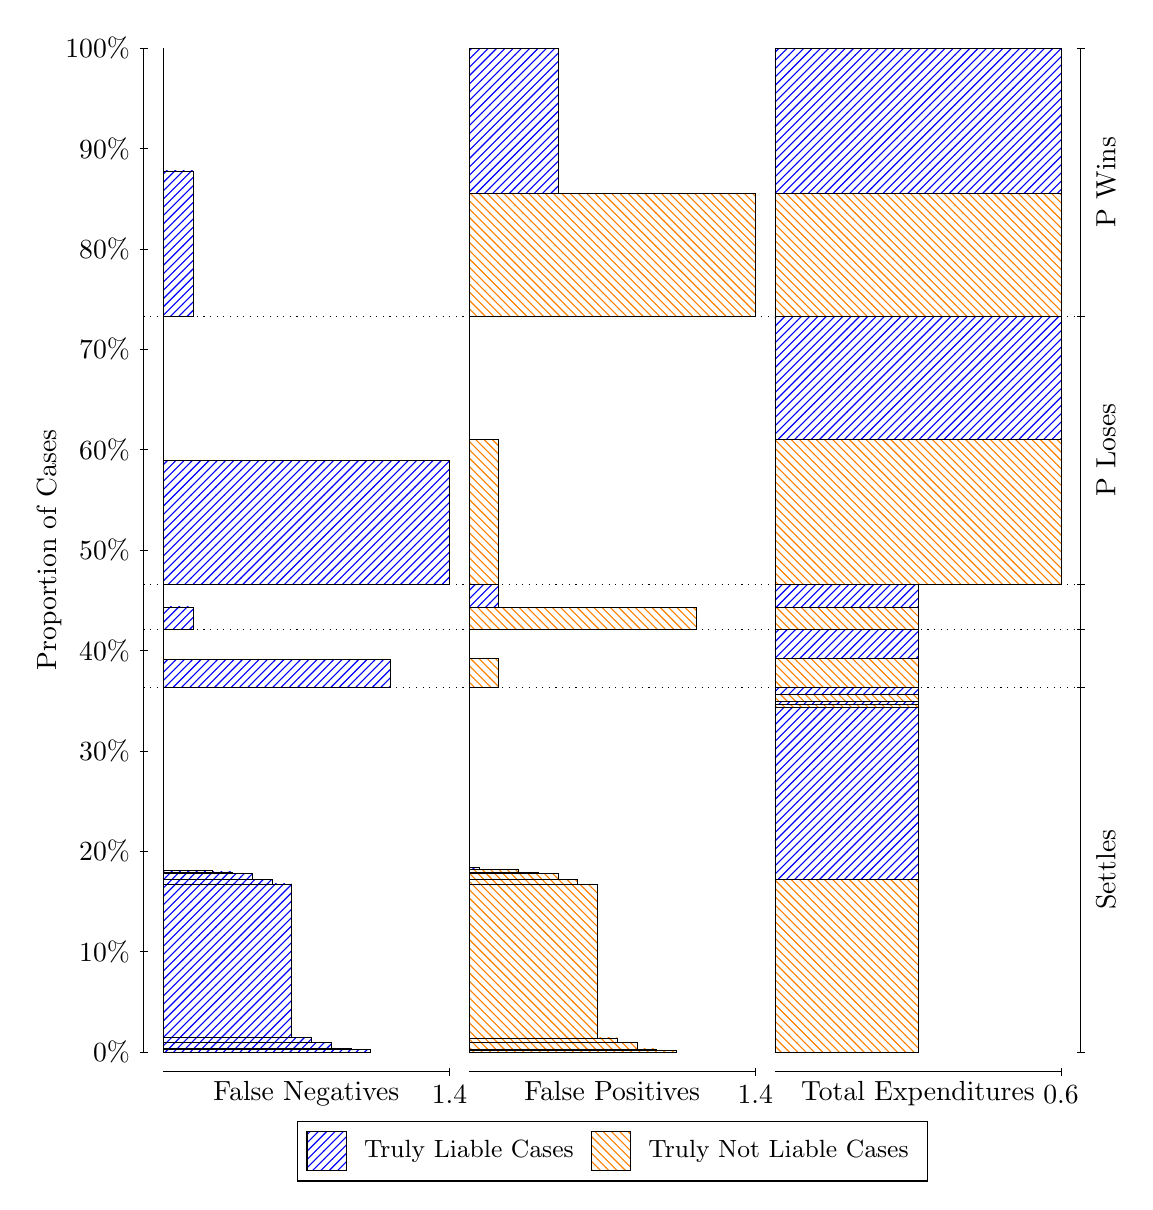
\begin{tikzpicture}
\draw[black, very thin] (1.5,1.75) -- (1.5,14.5);
\node[rotate=90, anchor=center] at (0.3, 8.125) {Proportion of Cases};
\draw[black, very thin] (1.45,1.75) -- (1.55,1.75);
\node[anchor=east] at (1.45, 1.75) {0\%};
\draw[black, very thin] (1.45,3.025) -- (1.55,3.025);
\node[anchor=east] at (1.45, 3.025) {10\%};
\draw[black, very thin] (1.45,4.3) -- (1.55,4.3);
\node[anchor=east] at (1.45, 4.3) {20\%};
\draw[black, very thin] (1.45,5.575) -- (1.55,5.575);
\node[anchor=east] at (1.45, 5.575) {30\%};
\draw[black, very thin] (1.45,6.85) -- (1.55,6.85);
\node[anchor=east] at (1.45, 6.85) {40\%};
\draw[black, very thin] (1.45,8.125) -- (1.55,8.125);
\node[anchor=east] at (1.45, 8.125) {50\%};
\draw[black, very thin] (1.45,9.4) -- (1.55,9.4);
\node[anchor=east] at (1.45, 9.4) {60\%};
\draw[black, very thin] (1.45,10.675) -- (1.55,10.675);
\node[anchor=east] at (1.45, 10.675) {70\%};
\draw[black, very thin] (1.45,11.95) -- (1.55,11.95);
\node[anchor=east] at (1.45, 11.95) {80\%};
\draw[black, very thin] (1.45,13.225) -- (1.55,13.225);
\node[anchor=east] at (1.45, 13.225) {90\%};
\draw[black, very thin] (1.45,14.5) -- (1.55,14.5);
\node[anchor=east] at (1.45, 14.5) {100\%};

\draw[black, very thin] (13.4,1.75) -- (13.4,14.5);
\draw[black, very thin] (13.35,1.75) -- (13.45,1.75);
\node[anchor=west] at (13.35, 1.75) {};
\draw[black, very thin] (13.35,6.3788) -- (13.45,6.3788);
\node[anchor=west] at (13.35, 6.3788) {};
\draw[black, very thin] (13.35,7.112) -- (13.45,7.112);
\node[anchor=west] at (13.35, 7.112) {};
\draw[black, very thin] (13.35,7.6907) -- (13.45,7.6907);
\node[anchor=west] at (13.35, 7.6907) {};
\draw[black, very thin] (13.35,11.094) -- (13.45,11.094);
\node[anchor=west] at (13.35, 11.094) {};
\draw[black, very thin] (13.35,14.5) -- (13.45,14.5);
\node[anchor=west] at (13.35, 14.5) {};

\draw[black, very thin, pattern color=blue, pattern=north east lines] (1.75,1.75) rectangle (4.381,1.7865);
\draw[black, very thin, pattern color=blue, pattern=north east lines] (1.75,1.7865) rectangle (4.1305,1.7979);
\draw[black, very thin, pattern color=blue, pattern=north east lines] (1.75,1.7979) rectangle (3.8799,1.8709);
\draw[black, very thin, pattern color=blue, pattern=north east lines] (1.75,1.8709) rectangle (3.6293,1.9341);
\draw[black, very thin, pattern color=blue, pattern=north east lines] (1.75,1.9341) rectangle (3.3787,3.8842);
\draw[black, very thin, pattern color=blue, pattern=north east lines] (1.75,3.8842) rectangle (3.1282,3.9429);
\draw[black, very thin, pattern color=blue, pattern=north east lines] (1.75,3.9429) rectangle (2.8776,4.0188);
\draw[black, very thin, pattern color=blue, pattern=north east lines] (1.75,4.0188) rectangle (2.627,4.0382);
\draw[black, very thin, pattern color=blue, pattern=north east lines] (1.75,4.0382) rectangle (2.3764,4.0593);
\draw[black, very thin, pattern color=orange, pattern=north west lines] (1.75,4.0593) rectangle (1.75,6.3788);
\draw[black, very thin, pattern color=blue, pattern=north east lines] (1.75,6.3788) rectangle (4.6316,6.7388);
\draw[black, very thin, pattern color=orange, pattern=north west lines] (1.75,6.7388) rectangle (1.75,7.112);
\draw[black, very thin, pattern color=blue, pattern=north east lines] (1.75,7.112) rectangle (2.1259,7.4017);
\draw[black, very thin, pattern color=orange, pattern=north west lines] (1.75,7.4017) rectangle (1.75,7.6907);
\draw[black, very thin, pattern color=blue, pattern=north east lines] (1.75,7.6907) rectangle (5.3833,9.2592);
\draw[black, very thin, pattern color=orange, pattern=north west lines] (1.75,9.2592) rectangle (1.75,11.094);
\draw[black, very thin, pattern color=blue, pattern=north east lines] (1.75,11.094) rectangle (2.1259,12.941);
\draw[black, very thin, pattern color=orange, pattern=north west lines] (1.75,12.941) rectangle (1.75,14.5);
\draw[black, very thin, pattern color=orange, pattern=north west lines] (5.6333,1.75) rectangle (8.2644,1.7703);
\draw[black, very thin, pattern color=orange, pattern=north west lines] (5.6333,1.7703) rectangle (8.0138,1.7905);
\draw[black, very thin, pattern color=orange, pattern=north west lines] (5.6333,1.7905) rectangle (7.7632,1.8684);
\draw[black, very thin, pattern color=orange, pattern=north west lines] (5.6333,1.8684) rectangle (7.5126,1.9284);
\draw[black, very thin, pattern color=orange, pattern=north west lines] (5.6333,1.9284) rectangle (7.2621,3.8812);
\draw[black, very thin, pattern color=orange, pattern=north west lines] (5.6333,3.8812) rectangle (7.0115,3.9439);
\draw[black, very thin, pattern color=orange, pattern=north west lines] (5.6333,3.9439) rectangle (7.0115,3.9458);
\draw[black, very thin, pattern color=orange, pattern=north west lines] (5.6333,3.9458) rectangle (6.7609,4.0199);
\draw[black, very thin, pattern color=orange, pattern=north west lines] (5.6333,4.0199) rectangle (6.5103,4.0312);
\draw[black, very thin, pattern color=orange, pattern=north west lines] (5.6333,4.0312) rectangle (6.2598,4.0695);
\draw[black, very thin, pattern color=blue, pattern=north east lines] (5.6333,4.0695) rectangle (5.7586,4.0906);
\draw[black, very thin, pattern color=blue, pattern=north east lines] (5.6333,4.0906) rectangle (5.6333,6.3788);
\draw[black, very thin, pattern color=orange, pattern=north west lines] (5.6333,6.3788) rectangle (6.0092,6.752);
\draw[black, very thin, pattern color=blue, pattern=north east lines] (5.6333,6.752) rectangle (5.6333,7.112);
\draw[black, very thin, pattern color=orange, pattern=north west lines] (5.6333,7.112) rectangle (8.5149,7.401);
\draw[black, very thin, pattern color=blue, pattern=north east lines] (5.6333,7.401) rectangle (6.0092,7.6907);
\draw[black, very thin, pattern color=orange, pattern=north west lines] (5.6333,7.6907) rectangle (6.0092,9.5251);
\draw[black, very thin, pattern color=blue, pattern=north east lines] (5.6333,9.5251) rectangle (5.6333,11.094);
\draw[black, very thin, pattern color=orange, pattern=north west lines] (5.6333,11.094) rectangle (9.2667,12.653);
\draw[black, very thin, pattern color=blue, pattern=north east lines] (5.6333,12.653) rectangle (6.7609,14.5);
\draw[black, very thin, pattern color=orange, pattern=north west lines] (9.5167,1.75) rectangle (11.333,3.9439);
\draw[black, very thin, pattern color=blue, pattern=north east lines] (9.5167,3.9439) rectangle (11.333,6.1305);
\draw[black, very thin, pattern color=orange, pattern=north west lines] (9.5167,6.1305) rectangle (11.333,6.1688);
\draw[black, very thin, pattern color=blue, pattern=north east lines] (9.5167,6.1688) rectangle (11.333,6.2053);
\draw[black, very thin, pattern color=orange, pattern=north west lines] (9.5167,6.2053) rectangle (11.333,6.2926);
\draw[black, very thin, pattern color=blue, pattern=north east lines] (9.5167,6.2926) rectangle (11.333,6.3788);
\draw[black, very thin, pattern color=orange, pattern=north west lines] (9.5167,6.3788) rectangle (11.333,6.752);
\draw[black, very thin, pattern color=blue, pattern=north east lines] (9.5167,6.752) rectangle (11.333,7.112);
\draw[black, very thin, pattern color=orange, pattern=north west lines] (9.5167,7.112) rectangle (11.333,7.401);
\draw[black, very thin, pattern color=blue, pattern=north east lines] (9.5167,7.401) rectangle (11.333,7.6907);
\draw[black, very thin, pattern color=orange, pattern=north west lines] (9.5167,7.6907) rectangle (13.15,9.5251);
\draw[black, very thin, pattern color=blue, pattern=north east lines] (9.5167,9.5251) rectangle (13.15,11.094);
\draw[black, very thin, pattern color=orange, pattern=north west lines] (9.5167,11.094) rectangle (13.15,12.653);
\draw[black, very thin, pattern color=blue, pattern=north east lines] (9.5167,12.653) rectangle (13.15,14.5);
\draw[black, dotted] (1.5,6.3788) -- (13.4,6.3788);
\draw[black, dotted] (1.5,7.112) -- (13.4,7.112);
\draw[black, dotted] (1.5,7.6907) -- (13.4,7.6907);
\draw[black, dotted] (1.5,11.094) -- (13.4,11.094);
\draw[black, very thin] (1.75,1.5) -- (5.3833,1.5);
\node[anchor=north] at (3.5667, 1.5) {False Negatives};
\draw[black, very thin] (5.3833,1.45) -- (5.3833,1.55);
\node[anchor=north] at (5.3833, 1.45) {1.4};

\draw[black, very thin] (5.6333,1.5) -- (9.2667,1.5);
\node[anchor=north] at (7.45, 1.5) {False Positives};
\draw[black, very thin] (9.2667,1.45) -- (9.2667,1.55);
\node[anchor=north] at (9.2667, 1.45) {1.4};

\draw[black, very thin] (9.5167,1.5) -- (13.15,1.5);
\node[anchor=north] at (11.333, 1.5) {Total Expenditures};
\draw[black, very thin] (13.15,1.45) -- (13.15,1.55);
\node[anchor=north] at (13.15, 1.45) {0.6};

\node[black, centered, rotate=90] at (13.72, 4.0644) {Settles};


\node[black, centered, rotate=90] at (13.72, 9.3921) {P Loses};
\node[black, centered, rotate=90] at (13.72, 12.797) {P Wins};

\draw (7.449999999999999,1.5) node[draw=none] (baseCoordinate) {};
\begin{scope}[align=center]
        \matrix[scale=0.5, draw=black, below=0.5cm of baseCoordinate, nodes={draw}, column sep=0.1cm]{
            \node[rectangle, draw, minimum width=0.5cm, minimum height=0.5cm, pattern=north east lines, pattern color=blue] {}; &
            \node[draw=none, font=\small] (B) {Truly Liable Cases}; &
            \node[rectangle, draw, minimum width=0.5cm, minimum height=0.5cm, pattern=north west lines, pattern color=orange] {}; &
            \node[draw=none, font=\small] (B) {Truly Not Liable Cases}; \\
            };
\end{scope}

\end{tikzpicture}
\end{document}